\documentclass[]{beamer}
\usetheme{KUL}
\usepackage{multirow}
\usepackage{multicol}
\usepackage{tikz}
\usepackage{ulem}
\usepackage{todonotes}
\usepackage{siunitx}
\newcommand\itemS{\item[\textbf{\S}]}
\definecolor{darkgreen}{rgb}{0,0.598,0.199}
\usepackage{times} % set font on times new roman
\usepackage{eurosym} % package for Euro sign
\usepackage{lineno}   % package for line numbering
\usepackage{hyperref} % this is for url links
\usepackage{subcaption}  % this package enables one to put several figures next to each other
\usepackage{textcomp}
\usepackage{setspace}
\usepackage{gensymb}
\usepackage{tikz}
\usetikzlibrary{positioning}
\usetikzlibrary{matrix, arrows, graphs}
\usetikzlibrary{backgrounds}
\usetikzlibrary{calc}
\usepackage{amsmath}
\usepackage{adjustbox}
\usepackage[absolute,overlay]{textpos}


\title{Thesis}
\subtitle{Building A Secure and Open \\ IoT Platform with ARM TrustZone}
\author{Oberon Swings}
\institute{KU Leuven}
\date{\today}


\setbeamercolor{framesource}{fg=gray}
\setbeamerfont{framesource}{size=\tiny}
\newcommand{\source}[1]{\begin{textblock*}{0.4\textwidth}(0.75\textwidth ,0.8\textwidth)
    \begin{beamercolorbox}[ht=0cm,right]{framesource}
        \usebeamerfont{framesource}\usebeamercolor[fg]{framesource} {#1}
    \end{beamercolorbox}
\end{textblock*}}



\begin{document}

{
		\setbeamertemplate{headline}{} %define local, empty header for title page
		\setbeamertemplate{footline}{} %define local, empty footer for title page
		\source{image: https://developer.arm.com/ip-products/security-ip/trustzone}
		\maketitle
	}
	\addtocounter{framenumber}{-1} % We don't count the title page
	
\iftrue
% Table of Contents
\begin{frame}{Outline}
	\hfill	{\large \parbox{.95\textwidth}{\tableofcontents[hideothersubsections]}}
\end{frame}
\fi

\section{Secure Open Platform}

\begin{frame}{Goals}
\begin{columns}
\column{0.55\textwidth}
\begin{itemize}
% An open IoT platform is the middleware between the hardware of the IoT device and the software that is put on there by the software providers.
\item Middleware
% These platforms are used to connect to IoT devices, manage these devices and support data analysis. There are lots of other capabilities these platforms provide. 
\item Connect, manage, support,...
%
\item Openness \begin{itemize}
\item Open-source
\item Open standards
\item Open APIs
% data needs to be accessible by everyone to use and republish, so there are no restrictions from copyright or similar constructions. 
\item Open data
% open software layer, this is often achieved through the open APIs
\item Open layer
\end{itemize}
\end{itemize}
\column{0.5\textwidth}
\begin{figure}
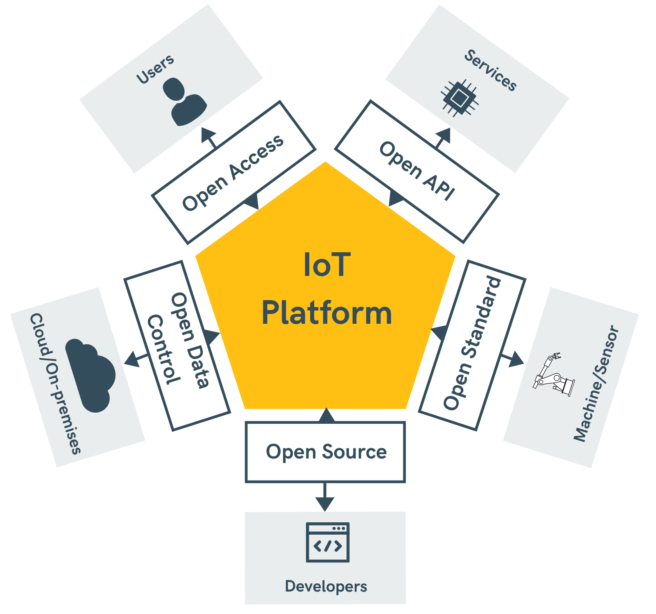
\includegraphics[width=1\textwidth]{Pictures/open-IoT-platform.png}
\end{figure}
\end{columns}
\source{image: https://www.record-evolution.de/en/what-is-an-open-iot-platform-and-why-use-one/}
\end{frame}

\begin{frame}{Problems}
\begin{itemize}
% Shared resources have the problem that they could be accessed by others
\item Shared resources \begin{itemize}
\item I/O
\item Memory
\item CPU
\end{itemize}
% The software providers don't necessarily trust eachother or the operating system
\item Lack of trust \begin{itemize}
\item Software providers
\item Operating system
\end{itemize}
\end{itemize}
\end{frame}

\begin{frame}{Security}
\begin{itemize}
% software isolation ensures that software modules of a provider don't interfere with those of others
\item Software isolation
% secure IO makes sure that other software doesn't interfere with the IO of an application
\item Secure I/O
% secure communication is similar to secure IO but more specifically focussed on communication between modules
\item Secure communication
% remote attestation can prove to the software provider that their software modules have not been tampered with
\item Remote attestation
\end{itemize}
\end{frame}

\section{ARM TrustZone}

\begin{frame}{Trusted Execution Environment}
\begin{itemize}
% a trusted execution environment is based on a secure execution environment in addition with trust. This trust is often achieved through remote attestation that can prove the trustworthyness for third parties.
\item TEE (Trusted Execution Environment) \begin{itemize}
\item Authenticity (execution)
\item Confidentiality (states)
\item Integrity (code and data)
\item Minimize TCB
\end{itemize}
\end{itemize}
\end{frame}

\begin{frame}{Implementation}
\begin{itemize}
% ARM TrustZone is hardware-based security built into the system on chip to provide a basis for improved system security
\item Processor level vs OS level (Intel SGX)
% The processor has two main execution environments, these are the normal and secure worlds. 
\item Secure and normal world
% The isolation between these worlds is enforced by hardware. The processor saves the register states for instance and reloads them to the correct state during a world switch, this ensures that the normal world can never access data owned by the secure world.
\item Hardware isolation
% In memory this differentiation has also been made by the TZASC, it enables to tag memory regions as secure or normal.
\item TrustZone Address Space Controller
\end{itemize}
\end{frame}

\begin{frame}{Root of Trust}
\begin{columns}
\column{0.45\textwidth}
\begin{itemize}
% When trying to achieve built-in trust, this trust has to come from somewhere.
\item Chain of trust \begin{itemize}
% A secure application is only secure if the assumptions made are also met
\item Secure application
% One of these assumptions is that the Trusted Execution Environment framework it uses works correctly (most importantly is not tampered with)
\item TEE framework
% The tee framework itself also assumes that it has been started up from a secure place, if the booting process for instance was tampered with the framework can still be bypassed
\item Booting process
% The booting process can in turn be secured with a secure module which is available on certain hardware. This piece of hardware is seen as the root of trust or is used to achieve the root of trust. for instance by having a byte array stored on it which is the input to a hash algorithm which in turn is the root of trust of the system.
\item Secure module
\end{itemize}
% The root of the trust chain is not a perfectly secure entity, it is assumed though that it is very hard to break or that trying to tamper with it destroys it for instance.
\item Root of trust
\end{itemize}
\column{0.55\textwidth}
\begin{figure}
\includegraphics[width=1\textwidth]{Pictures/chainofTrust.jpg}
\end{figure}
\end{columns}
\source{image: https://www.phaedsys.com/principals/ iconlabs/Iconfloodgatesecureboot.html}
\end{frame}

\section{PinePhone}

\begin{frame}{Hardware}
\begin{figure}
% These are the high level specs of the PinePhone, the most important ones for this thesis are the Allwinner A64 which has an ARM TrustZone enables SoC. The second important aspect of the phone is that it can be booted using a bootable microSD card.
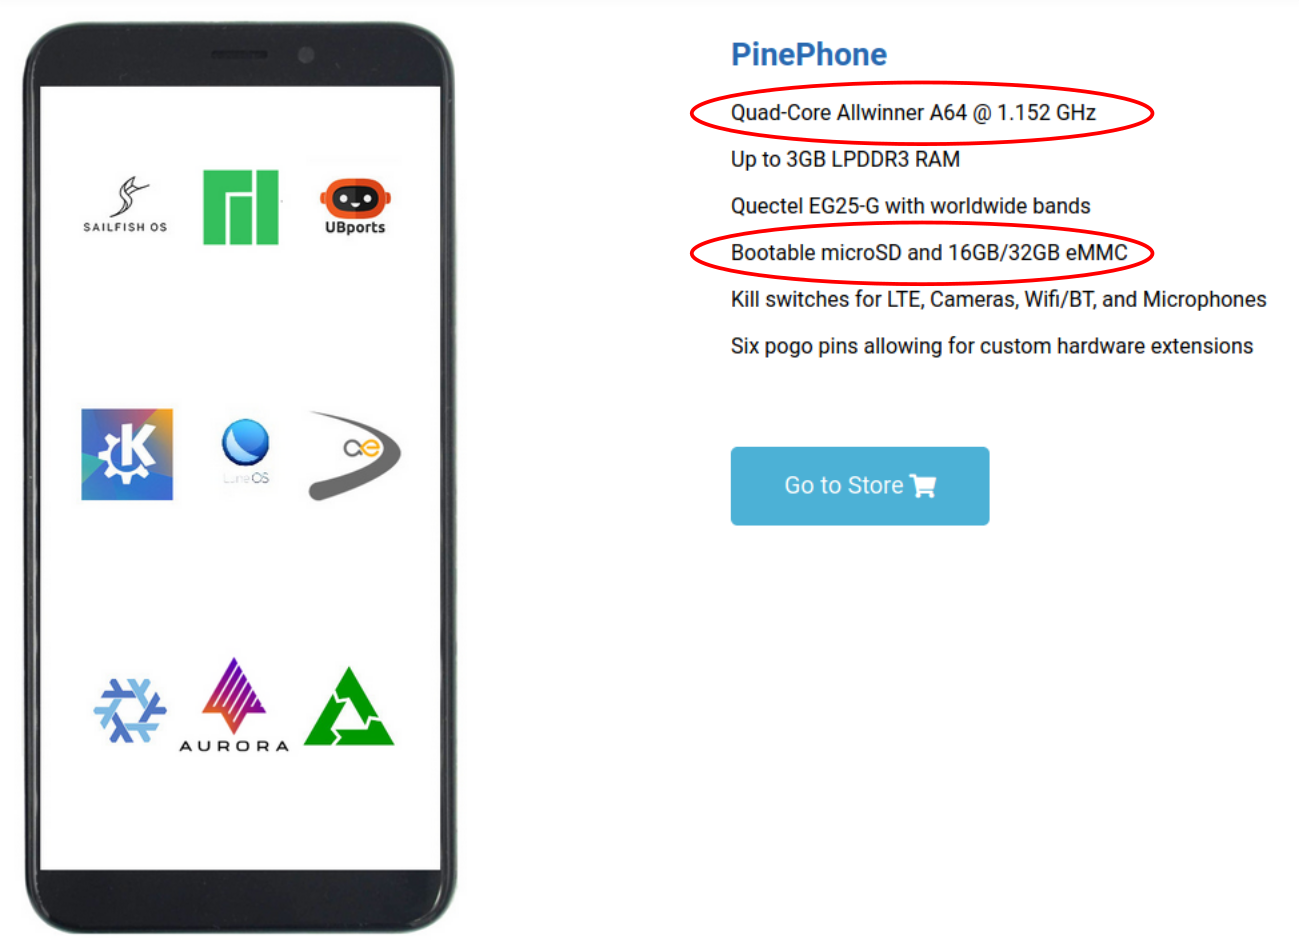
\includegraphics[width=0.8\textwidth]{Pictures/pinephone-specs.png}
\end{figure}
\source{image: https://www.pine64.org/pinephone/}
\end{frame}

\begin{frame}{Application}
\begin{itemize}
% The PinePhone is an open source smartphone which can be turned into an open IoT platform
\item Open-source smartphone \begin{itemize}
\item Open standards
\item Open data
\end{itemize}
% The second aspect is that it is a Linux phone which gives great advantages towards experimenting with the device and adds to the open APIs and open source aspect of the open platform.
\item Linux \begin{itemize}
\item Open source
\item Open APIs
\end{itemize}
% With these aspects in mind, it seems that the pinephone could be turned into a nice open platform for mobile computing
\item Open platform for mobile computing
\end{itemize}
\end{frame}

\begin{frame}{OP-TEE}
\begin{itemize}
% OP-TEE stands for Open Portable Trusted Execution Environment.
\item Open Portable Trusted Execution Environment
% It is a framework which implements security solutions based on the features ARM TrustZone provides.
\item Relies on ARM TrustZone
% There are two main components in OP-TEE namely the client which interacts with the rich OS and the optee OS which interacts with the ARM TrustZone primitives.
\item Client and OS
% The rich OS in the case of optee is often a Linux based operating system.
\item Interacts with Linux 

\end{itemize}
\end{frame}

\section{Research}

\begin{frame}{Research Questions}
Can the PinePhone be turned into a secure open IoT platform?
\begin{itemize}
\item What security features from OP-TEE are necessary to achieve a secure open platform on the PinePhone?
\item Is it feasible to secure boot the PinePhone, and in this way achieve a root of trust?
\item Can the I/O of the PinePhone be secured using OP-TEE and ARM TrustZone?
\end{itemize}
\end{frame}

\begin{frame}{Hypothesis}
\begin{itemize}
\item OP-TEE can be ported onto a PinePhone and will atleast enable ARM TrustZone and secure boot.
\item The secure boot will ensure that OP-TEE is started from a secure and trusted space ensuring it will work correctly.
\item Secure applications will be able to make use of ARM TrustZone through OP-TEE and in this way achieve secure I/O on the device.
\end{itemize}
\end{frame}

\section{Progress}

\begin{frame}{Past}
\begin{itemize}
\item Literature study
\item Qemu emulator
\item Secure applications
\item AuthenticExecution framework
\end{itemize}
\end{frame}

\begin{frame}{Present}
\begin{columns}
\column{0.4\textwidth}
\begin{itemize}
\item Booting PinePhone with OP-TEE
\end{itemize}
\column{0.6\textwidth}
\begin{figure}
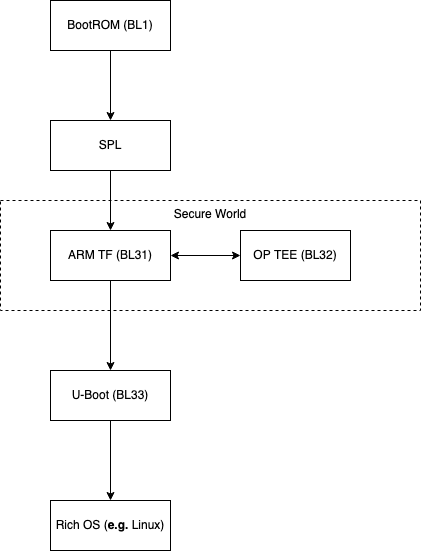
\includegraphics[width=0.8\textwidth]{Pictures/ARMv8_BootFlow.png}
\end{figure}
\end{columns}
\source{image: https://mquaresma.github.io/pine/a64/ 2020/04/11/Setting-up-OPTEE-and-Linux-for-the-Pine-A64.html}
\end{frame}

\begin{frame}{Future}
\begin{itemize}
\item Tweak booting for secure boot
\item Proof of concept for secure I/O
\item Write thesis
\end{itemize}
\end{frame}

\part{}

\begin{frame}{Questions?}
\begin{figure}
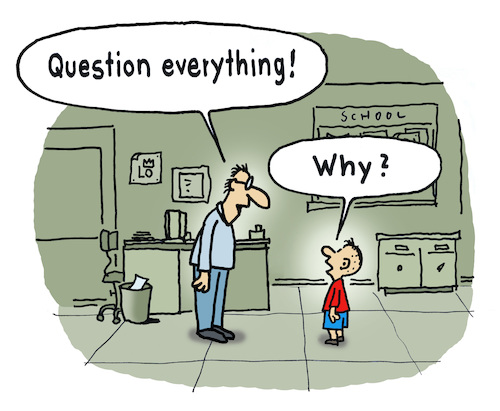
\includegraphics[width=0.7\textwidth]{Pictures/questions.jpg}
\end{figure}
\source{image: https://www.toonpool.com/cartoons/ Question\_376876}
\end{frame}


\end{document}